\documentclass[10pt,conference,compsocconf]{IEEEtran}

\usepackage{hyperref}
\usepackage{graphicx}
\usepackage[]{algorithm2e}
\usepackage{placeins}
\usepackage[english]{babel}
\usepackage[usenames, dvipsnames]{color}

\begin{document}
\title{Machine Learning -- Project 2}
\author{
 Alexander Holloway -- Bastian Nanchen -- Arnaud Pannatier 
  \\
  \textit{Group : }Max and Lily learn ML \\
  \textit{EPFL 2017}
}
\maketitle

\begin{abstract}
Sentiment classification is an active area of research in the field of machine learning. Here, we present the results of a study into supervised learning methods for classifying the emotional sentiment of Tweets -- either positive, or negative -- according to the presence of an emoticon. To this end, we leverage state-of-the-art pre-processing and feature engineering methods, and provide a comparison of learning methods that make use of the resultant features. Finally, we describe in detail the best model we identified for this purpose: Convolutional neural network with dropout layer, which achieved 82.6\% accuracy on unseen data.
\end{abstract}

\section{Data}
\label{sec:data}

The data supplied through the online competition platform consists of 2.5 million labelled training examples, which take the form of Tweets that previously contained either positive or negative emoticons. The dataset is split down the middle, with 1.25 million training examples available for each class---positive and negative. Contrary to other similar classification tasks presented in the literature \cite{jiang2011target, tang2014learning}, there are no ``neutral'' class labels in this dataset. The absence of such indeterminate class labels allows us to formulate this problem as a binary classification task, which is advantageous.

Due to the nature of the Twitter platform, the dataset contains many ``words'' that do not belong in a tradition English lexicon. Examples of these are usernames, URLs, hashtags, colloquialisms or slang, and even typographical errors (both intentional and unintentional). Usernames and URLs were already stripped from the data, however the presence of other artefacts poses both issues and opportunities for this classification task. For example, the presence of repeated punctuation marks or characters may not make syntactic sense in trational language, but more often than not has semantic meaning within a Tweet \cite{tang2014learning}. Similarly, hashtags can provide significant predictive power for the sentiment of phrase, without containing meaning in a traditional pragmatic sense.

A detailed explanation of the specific language artefacts we processed, and the ways in which we leveraged them to improve classification performnce is presented in Section \ref{sec:processing}.


\section{Feature processing}
\label{sec:processing}
In order to train learning models using the Twitter data, it was necessary to perform pre-processing to create useful features that characterise the two classes we seek to disambiguate. The dataset that was provided include some basic preprocessing but additional transformation were performed in order to improve our classification performance. Some transformations are inspired by the Glove documentation \cite{Glove}. 

\subsection{Base transformations}
Each line of the provided data files represents one Tweet, with all words separated by a single whitespace. All URLs have been removed, and mentions of other users are replaced by the tag \texttt{<user>}. Necessarily, all emoticons have also been removed, however there is no indication of their presence within the original Tweet.

\subsection{Number transformation}
The idea is that all the numbers contained in a tweet have the same meaning for sentiment analysis. Therefore it makes sense to group them. To do that all the numbers are replaced with a tag: \texttt{<NUMBER>}

\subsection{Hashtag splitting}
The hashtag part of the tweet is especially hard to process. For now most of the hashtag are treated as different words in the vocabulary. Of course, if the program manages to split them the right way, it will add a lot of understanding for the machine. A basic idea was to replace the \# by the tag \texttt{<HASHTAG>} and then split all the words on uppercase letters. Sometimes the hashtag are in uppercase, Obviously in that case, the hashtag shouldn't be splited. So all the words are kept like that and an additionnal \texttt{<ALLCAPS>} is added at the end of the hashtag. For example the hashtag \texttt{\#ILikeMachineLearning} will be transformed in \texttt{<HASHTAG> I Like Machine Learning} and \texttt{\#ILIKEMACHINELEARNING} will be transformed in \texttt{<HASHTAG> ILIKEMACHINELEARNING <ALLCAPS>}. 

\subsection{Punctuation repetitions}
Sometimes the punctuation is repeated at the ends of words. As before, it's more convenient to treat an expression like \texttt{!!!!!} the same way that \texttt{!!!} and not as two differents words. Therefore each time a punctuation mark is repeated, it is transformed in \texttt{punctuation mark <REPEAT>}. 

\subsection{Elongated words}
In some tweets the last letter of some words is repeated. This is a similar problem than before. All these expressions should be treated as the same word in the vocabulary. In order to do so, all the repeated letters at the end of a word are replaced be \texttt{word without repetition <ELONG>}.

\section{Classification methods}
Using the generated features 4 methods are applied to classify the data between happy tweets and sad ones. The three first are classic feature classifications that were applied to the tweets features. The last one is a more complex classification method and is directly applied on the embeddings.

\subsection{Logistic regression}
The first classifier that is applied is standard logistic regression. This classifier use the logistic function to determines whether the tweets belongs to one categories or another. This really simple method as the advantage that it is really fast to compute and easy to implement. It can be use to determine if the modification of the data processing as an impact on classification. But it will not be efficient enough to use for the competitions.

\subsection{SVM}
The more advanced classification technic of \textit{Support vector machine} is implemented as well. This method is often use in supervised learning. Given a set of training example belonging to two different categories, the SVM model build a frontier between the samples of the two categories with the biggest gap possible. This technics leads to better results for classification but also takes more times to run. 

\begin{figure}[h!]
\centering
	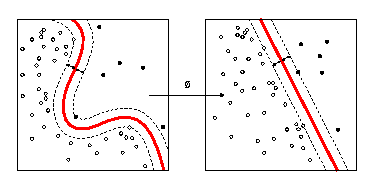
\includegraphics[scale=1.2]{SVM} 
\caption{The SVM model tries to find the frontier with the bigger gap possible.}
\label{plot:SVM}
\end{figure}
\FloatBarrier

\subsection{Regular neural networks}

Neural nets were also used on tweets features. This neural net has two layers of size TODO COMPLETE: (..,..). This was to take account that a neural network of  two layers is sufficient to represent any vectorial function.  If this technic was giving the best results of all the one that were used on on tweets representation, it didn't lead to the sufficiently good results for the competition. 

\subsection{Convolutional neural networks}

In order to achieve better classification, a convolutional neural network is applied. The idea is not just to look as the tweet as a vectorial sum of embeddings, but to consider their places in the tweets as well. In this case, all the tweets are represented by a matrix :  At each word of the tweet corresponds a line of the matrix, containing the embeddings of the words. This matrix has therefore a size of \texttt{(number of words in the tweet * dimension of embeddings)}. A first layer apply then the convolution, it creates some filters of given sizes (in our case 3,4,5), which will be slided over the tweets matrix. 


\begin{figure}[h!]
\centering
	\includegraphics[scale=0.3]{CNN} 
\caption{Model of the convolutional neural network used for sentiment analysis}
\label{plot:CNN}
\end{figure}

\label{sec:methods}

\section{Results}
Classification performances measured in local hold-out testing are presented for each of the methods are presented in Table \ref{tab:results}. Precision, recall and accuracy were computed on a hold-out split where 2.4 million examples were used for training, and the remaining 100 thousand samples were evaluated for testing.

\begin{table}[h]
  \centering
  \begin{tabular}[c]{lllll}
    Input format&Model&Accuracy&Precision&Recall\\
    \hline
    Tweet-embed.&Logistic regression & 60.60 &    60.84   & 60.64  \\
    Tweet-embed.&SVM             & 61.96    &   63.69     & 62.05   \\
    Tweet-embed.&Neural network & 65.45	& 67.04	& 65.53	 \\
    Word-embed.&CNN w/o dropout &  81.12  & 81.80	& 81.75	 \\
    Word-embed.&CNN w/ dropout & 84.29 & 84.79 & 84.74

  \end{tabular}
  \caption{Classification performances using local hold-out testing, for various input data formats. Reported values are percentages.}
  \label{tab:results}
\end{table}

Initial exploration of classification performances indicated that the neural network models would provide better results than the simpler linear classifiers. For this reason, we chose to train these models for a greater number of epochs. The classification performance of two convolutional neural networks over successive training epochs can be seen in Figure \ref{plot:CNNaccuracy}. During the training process, the hold-out data was classified at the end of each epoch, and its performance was reported, allowing us to track improvements in classification performance over time.

\label{sec:results}
\begin{figure}[h!]
  \centering
  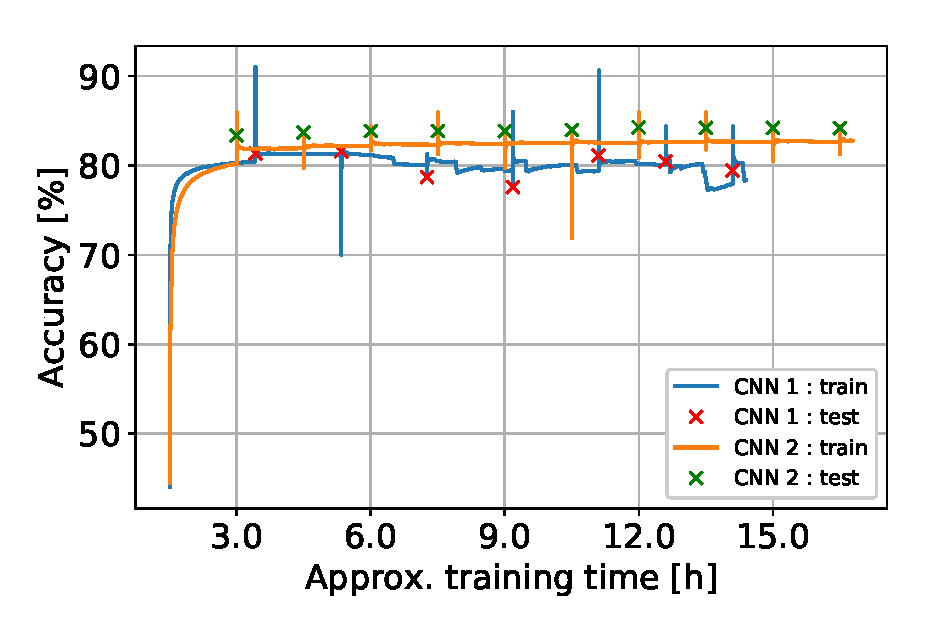
\includegraphics[scale=0.45]{CNNaccuracy}
  \caption{Hold-out classification accuracy over successive training epochs for two convolutional neural networks: CNN1 is a standard CNN, whereas CNN2 contains a dropout layer. Spikes in accuracy are caused by abberant values reported at the beginning of new epochs (indicated by crosses).}
  \label{plot:CNNaccuracy}
\end{figure}
\FloatBarrier

As expected, the convolutional network with a dropout layer was faster to train than without, allowing the model to be trained for further epochs. Furthermore, the regularizationinduced by the dropout layer yielded more accurate predictions. Extending the training time increased classification performance marginally, but naturally, perfomance plateaus at a certain point, after which additional training time has no benefit.

\section{Discussion}
\label{sec:discussion}

Here we have presented several methods of data pre-processing to create features from word-embeddings, and subsequently used these features to train a number of models. Empirically, we found that three different word-embeddings -- namely GloVe, skip-gram, and sentiment-specific -- gave comparable performance in the context of a Tweet sentiment classification task.

Classification performance was evaluated using four learning models: logistic regression, support vector machine, neural network, and convolutional neural network (CNN). Of these, all but the CNN took input in the form of word-embeddings which were aggregated per Tweet to create a so-called ``Tweet-embedding'' representation. The CNN accepted pre-trained word-embeddings that had not undergone such transformation, and in fact, achieved the best classification performance on an unseen test dataset.

There are many models for text classification outside of those explored here. Ultimately, classification performance on this task likely could be improved by using a pre-trained model (\emph{e.g.} Facebook's \texttt{fastText} \cite{joulin2016bag}), however, using a black box solution to maximise performance was not the aim of this project. When faced with similar tasks in the future, it would be illustrative to evaluate some of these ``out-of-the-box'' solutions, and explore their implementation details.


\bibliographystyle{IEEEtran}
\bibliography{report}

\end{document}
